\documentclass{article}
\usepackage{graphicx}
\usepackage{setspace}
\usepackage{booktabs}
%\usepackage{geometry}
\usepackage{titlesec}
\usepackage{fancyhdr}
\usepackage{subcaption}
\usepackage{microtype}
\usepackage{amsmath}
%\usepackage{breakurl}
\usepackage{minted}
\usepackage{helvet}
\usepackage[T1]{fontenc}
\usepackage{enumitem}
\usepackage{cite}
\usepackage{hyperref}
\usepackage{array}
\usepackage{tabularx}
\usepackage{minted}
\usepackage{xcolor}
\usepackage{caption}
\usepackage{multirow}
\usepackage{indentfirst}
\usepackage{subcaption}
\usepackage{multicol}
\usepackage{appendix}

\usepackage[letterpaper,top=2cm,bottom=2cm,left=3cm,right=3cm,marginparwidth=1.75cm]{geometry}

\begin{document}
\onehalfspacing
\begin{titlepage}
   \begin{center}
       \vspace*{7cm}
    \huge
       \textbf{Cloud Computing project documentation}
       \vspace{0.5 cm}
       \huge
       
        RealValuator: a web application for real estate appraisal 
       \vspace{1.5 cm}
    \large
    
       \textbf{Michał Binda, Aleksandra Kłos, Hubert Jaczyński}
       \vfill
    \large
       \vspace{0.7 cm}
    
       University Name: Warsaw University of Technology\\
       Department Name: Faculty of Mathematics and Information Science\\ 
       Date: 17th of April, 2025\\
            
   \end{center}
\end{titlepage}


\begin{titlepage}
   \begin{center}
       \vspace*{0.7 cm}
    \tableofcontents        
   \end{center}
\end{titlepage}


\section{Introduction}

In today's dynamically changing real estate market, developers, investors, and even individual clients are obliged to make decisions based on instant-available and precise data. Our web application, \textit{RealValuator}, offers an innovative solution that allows a comprehensive real estate valuation in real time. By integrating sophisticated machine learning algorithms and cloud data processing, the application's fundamental objective is to provide accurate property value forecasts based on the analysis of both historical data and current market trends.

 In this document, we would like to provide a business objective, technical design and implementation strategy for the \textit{RealValuator}. Precisely, the documentation covers the main motivation and features of the application, the high-level architecture - system diagram and roles of each major component, API design, containing the REST API endpoints, HTTP methods associated with each endpoint, the expected I/O data formats as well as error handling strategies. Furthermore, we will also delve into details of our chosen data storage solution. That is, we will explain why we have selected a structured SQL database over a NoSQL and the implementation details. Furthermore, we outline our approach to infrastructure management (IaC) using Terraform as well. In the final section, however, we establish the performance, availability, and latency targets for \textit{RealValuator}, defining SLA, SLO and SLI agreements. 


\section{Business goal}

\textit{RealValuator} application has been designed to improve the real estate valuation process by using new technologies that will be described in detail in the upcoming sections. The main business goal is to provide precise property value forecasts that will enable aforementioned users to make accurate investment decisions. The key objectives are as follows:

\begin{enumerate}
    \item The app uses historical market data analysis to generate precise property value forecasts. That is, users can rely on our results when making decisions about buying, selling, or investing in real estate.

    \item In times of dynamic market changes, it is necessary that data is available almost in real time. In order to react quickly and adapt investment strategies, \textit{RealValuator} provides instant query handling and clear presentation of results,

    \item To enable dynamic resource management, we have opted to implement a cloud solution, managed using tools such as Terraform. This makes the service scalable and minimizes infrastructure costs as resources are 'turned on' only when needed and 'turned off' during out-of-use periods.

    \item Thanks to comprehensive data analysis and an intuitive interface, RealValuator may help users understand market trends, assess the real value of real estate, and make decisions based on the provided data. Such a tool is especially useful in long-term investment planning and negotiation processes.
\end{enumerate}


\section{Architecture overview}

    \begin{figure}[h!]
    \centering
    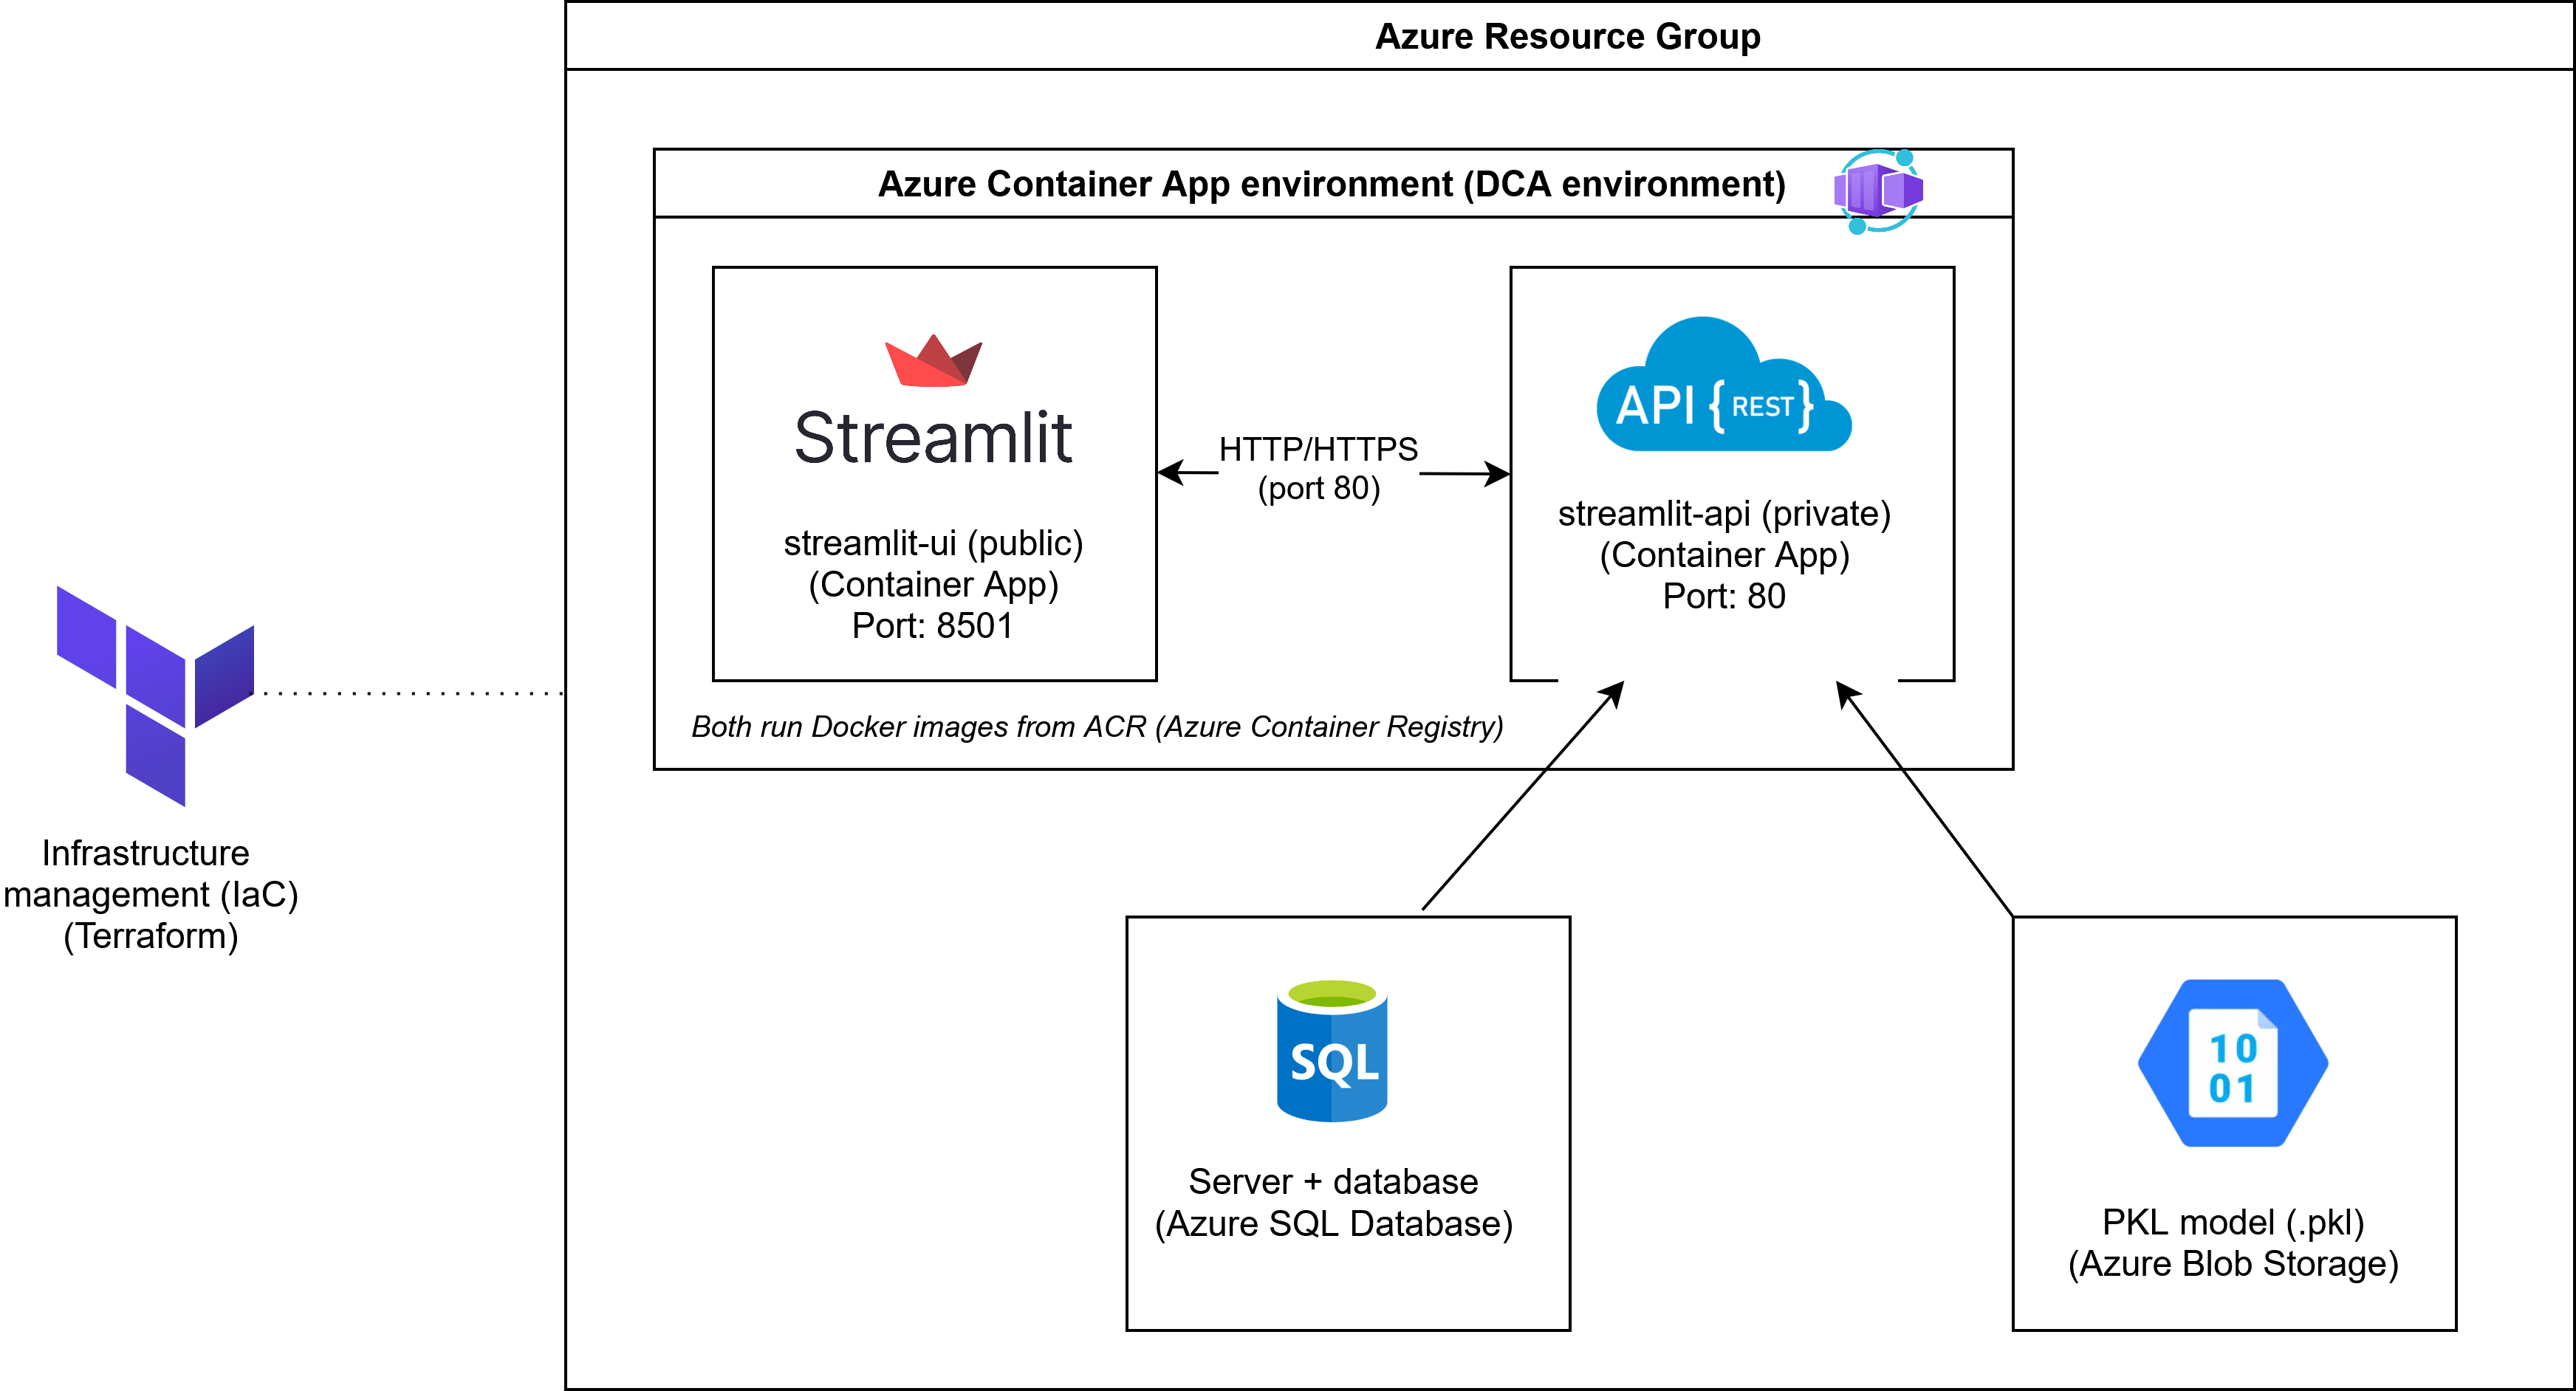
\includegraphics[width=12cm,keepaspectratio]{architecture.png}
    \caption{High-level architecture and data flow of the \textit{RealValuator} web application deployed on Azure. The diagram illustrates user input, API interaction, machine learning prediction using a serialized model, and infrastructure orchestration using Terraform.}
    \label{fig:arch}
\end{figure}


The diagram in Figure~\ref{fig:arch} illustrates the system architecture of the \textit{RealValuator}, which uses Microsoft Azure cloud services. This architecture was designed based on Platform-as-a-Service (PaaS) and serverless components, which allows for high flexibility, low operational costs, and ease of implementation. Furthermore, the infrastructure is managed by Terraform, which allows for automation, versioning, and reusability of environments (Infrastructure as Code – IaC). What is more, the entire application has been placed inside a single Azure Resource Group, with the idea of easier organization and resources monitoring.

\paragraph{}
The application workflow is presented in the following way:

\begin{enumerate}
    \item User interface 

The end-user uses the application via an intuitive interface created in Streamlit technology, running on Azure App Service. The user can enter property parameters, such as location, square footage, number of rooms etc., which are then passed to the backend. 

    
    \item API layer

After submitting the form, the data goes to the backend in the form of an HTTP (REST) request. This is handled by Azure Functions. The API layer is the central point of the system logic as it handles the data flow and controls subsequent operations.


    \item Operations on data 

This functionality reads and/or writes (saves) data from a SQL database -- Azure SQL Database which allows, among others, archiving queries, statistical analysis and input validation.
Simultaneously, the same data is transferred to the ML analytical module, which is responsible for calculating the projected value of the property of interest.

    \item ML/analytics module 

The ML/analytics module, written in Python, uses a pre-trained machine learning model saved as a .pkl file, a serialized model. This file is stored in Azure Blob Storage. Besides, the model is retrieved by the ML function, loaded into memory, and used to calculate the value of a property based on the input data.
    
    \item Results presentation

Once the prediction is made, the result is returned to the API layer and then sent back to the user interface, where it is presented in a user-friendly graphical form.

\end{enumerate}

\section{API design}

As mentioned previously, the interface is designed in a RESTful style, using Azure Functions services (HTTP-triggered) to handle requests. Below, the full specification is presented. It defines available endpoints, request and response formats, as well as error handling.  

\subsection{Endpoints description}

The application provides the following main endpoints:

\begin{itemize}
\item \textbf{\texttt{POST /predict}} – performs property value prediction. It accepts input data (city, square footage, number of rooms, floor etc.) in JSON format and returns the predicted value.
\item \textbf{\texttt{GET /status}} – checks the API status, returns the current status and timestamp.
\item \textbf{\texttt{GET /model-info}} – returns information about the currently used ML model, such as version, training date, accuracy and a list of used features.
\item \textbf{\texttt{GET /history}} – returns the history of user's queries.
\item \textbf{\texttt{POST /feedback}} – allows to send feedback from the user regarding the accuracy of the valuation.
\item \textbf{\texttt{DELETE /history/\{id\}}} – removes a particular record from the history, which can be useful from GDPR point of view.
\end{itemize}

\subsection{RealValuator specification}

The full specification in YAML format, describing all the API endpoints is presented as follows:

\begin{minted}[linenos, frame=lines, breaklines]{yaml}
info:
  title: RealValuator API
  version: "1.0.0"
  description: API for a cloud-based real estate valuation application.
servers:
  - url: https://localhost:7140/swagger/index.html
paths:
  /predict:
    post:
      summary: Predict property value.
      requestBody:
        required: true
        content:
          application/json:
            schema:
              type: object
              properties:
                address:
                  type: string
                  description: Street address of the property.
                city:
                  type: string
                  description: City where the property is located.
                area:
                  type: number
                  description: The total area of the property in square meters.
                rooms_number:
                  type: integer
                  description: The total number of rooms in the property.
                floor:
                  type: integer
                  description: The floor on which the property is located/ total number of floors in case of a house.
                year_built:
                  type: integer
                  description: The year the property was constructed.
              required:
                - address
                - city
                - area
                - rooms_number
                - floor
                - year_uilt
      responses:
        '200':
          description: Successful prediction response.
          content:
            application/json:
              schema:
                type: object
                properties:
                  estimated_value:
                    type: number
                  currency:
                    type: string
                  confidence:
                    type: number
        '400':
          description: Bad Request – Invalid input.
  /status:
    get:
      summary: Check API status.
      responses:
        '200':
          description: API is operational.
          content:
            application/json:
              schema:
                type: object
                properties:
                  status:
                    type: string
                  timestamp:
                    type: string
  /model-info:
    get:
      summary: Retrieve model metadata.
      responses:
        '200':
          description: Returns metadata for the ML model.
          content:
            application/json:
              schema:
                type: object
                properties:
                  model_version:
                    type: string
                  trained_on:
                    type: string
                  accuracy:
                    type: number
                  features:
                    type: array
                    items:
                      type: string
  /history:
    get:
      summary: Retrieve query history.
      parameters:
        - in: query
          name: user_id
          schema:
            type: string
          description: User identifier.
        - in: query
          name: limit
          schema:
            type: integer
          description: Maximum number of entries.
      responses:
        '200':
          description: Query history successfully retrieved.
          content:
            application/json:
              schema:
                type: array
                items:
                  type: object
                  properties:
                    address:
                      type: string
                    city:
                      type: string
                    area:
                      type: number
                    predicted:
                      type: number
                    timestamp:
                      type: string
  /feedback:
    post:
      summary: Submit user feedback regarding the prediction.
      requestBody:
        required: true
        content:
          application/json:
            schema:
              type: object
              properties:
                prediction_id:
                  type: string
                user_feedback:
                  type: string
                actual_price:
                  type: number
              required:
                - prediction_id
                - user_feedback
                - actual_price
      responses:
        '200':
          description: Feedback successfully recorded.
          content:
            application/json:
              schema:
                type: object
                properties:
                  status:
                    type: string
  /history/{id}:
    delete:
      summary: Delete a specific history record.
      parameters:
        - in: path
          name: id
          required: true
          schema:
            type: string
          description: Record identifier.
      responses:
        '200':
          description: Record deleted successfully.
          content:
            application/json:
              schema:
                type: object
                properties:
                  deleted_id:
                    type: string
                  status:
                    type: string
\end{minted}

\section{Storage characteristics}

This part of the documentation presents the characteristics of the data storage system, including the following aspects:

\subsection{Structured/ unstructed data}

In our application, key information such as property data (address, city, square footage, number of rooms, floor, year of construction) and valuation history are stored in tabular form. Due to the established structure (columns, data types, relations between tables), it might be possible to perform advanced queries, aggregations and reporting.

In the future, the system may also integrate unstructured data, such as system logs. However, for the current needs of the project, the main emphasis is placed on structured data, critical for prediction-making. 

\subsection{SQL/ NoSQL}

We have chosen Azure SQL Database, that is, a solution based on a relational database. This is because of the need to ensure strong data consistency. Data such as real estate information is fully structured, which allows for the use of SQL queries, indexing, and transactions (ACID properties). Additionally, thanks to it, complex analytical operations can be executed and integrated with other tools, for instance, reporting ones, in an effortless manner. 


\subsection{Strong/ Eventual consistency}

Due to the critical nature of real estate valuation data, where every transaction must be accurately recorded and retrieved later on, we employ strong consistency. The choice of relational database ensures that the data is available in an identical state to all users at all times, without an exception.

\subsection{Amount of data}

The system is designed to handle the medium-sized data typical of real estate appraisal applications. This includes:

\begin{enumerate}
    \item Input data for single valuations (several fields per record).
    \item Historical valuation records.
    \item Analytical data used to train and validate the ML model.
\end{enumerate}

As the system grows, the ability to scale the database is important. That is the reason why we choose a managed solution that allows for both vertical  -- increasing computing power, and horizontal scaling -- adding more resources if there would be such need.


\subsection{Read only/ Read \& write}

The main operations performed by the system include both reading data, such as retrieving information about a property, query history and writing like new entries regarding valuations or updating query history. The choice of a relational database ensures that these operations are performed along with maintaining consistency and transactional properties.

Furthermore, there are also parts of the system where read operations dominate, for example when retrieving ML model metadata or statistical data, but overall both of these operations are essential for our application to work as intended. 


\section{Terraform}

Throughout this project, infrastructure management is performed using Terraform, which allows defining cloud resources as code (Infrastructure as Code – IaC). We have chosen this solution due to several advantages:

\begin{enumerate}
    \item Terraform defines project resources as scripts, enabling automatic environment creation, infrastructure versioning, and minimizing manual configuration errors.
    \item The tool optimizes costs by enabling the start and shutdown of resources depending on our needs. For example, after completing work on some part of a project, we can easily shut down some elements, such as serveless services or databases. Therefore, as in many cloud solutions - we pay only for the resources we actively use. 
    \item Terraform implementation provides uniform and repeatable resource configuration, enabling rapid scaling and easy modification. As a best practice, it also enables integration with CI/CD processes to automatically update the environment during the application lifecycle. In this way, it increases control and consistency of the environment.
    \item Terraform configurations can incorporate security measures like using environment variables and configuration files for sensitive information storage and defining access policies using Role-Based Access Control (RBAC) to restrict resource permissions for unauthorized users.
\end{enumerate}

These bullet points clearly show us the most important features of the Terraform. This means that any environment employed can be quickly launched, configured and, if necessary, shut down without the loss of progress.  

\section{System agreements}

In order to guarantee high quality of services and user satisfaction, our system defines 3 key elements determining the level of services provided: SLA, SLO and SLI. They efine expected standards of availability, performance and quality of system operations, as well as they tend to establish appropriate mechanisms for monitoring and implementing possible reparatory actions.

\subsection{SLA}





\subsection{SLO}
\subsection{SLI}


\bibliographystyle{unsrt} 
\bibliography{bibliography}
\appendix



\end{document}

